\documentclass[10pt,a4paper,twocolumn]{article}
\usepackage[margin=17mm,top=16mm,bottom=17mm,columnsep=6.5mm]{geometry}
\usepackage[utf8]{inputenc}\usepackage[T1]{fontenc}\usepackage{mathptmx}\usepackage{microtype}
\usepackage{amsmath,amssymb,booktabs,graphicx,xcolor,enumitem,titlesec,balance}
\usepackage[font=small,labelfont=bf,skip=3pt]{caption}
\usepackage[numbers,sort&compress]{natbib}
\usepackage[hidelinks]{hyperref}
\graphicspath{{figs_v3/}}
\titleformat{\section}{\normalfont\bfseries\fontsize{10.5}{12}\selectfont}{\thesection}{0.6em}{}
\titleformat{\subsection}{\normalfont\bfseries\fontsize{10}{12}\selectfont}{\thesubsection}{0.6em}{}
\titlespacing*{\section}{0pt}{8pt plus 2pt}{3pt}\titlespacing*{\subsection}{0pt}{5pt plus 1pt}{2pt}
\setlist{nosep,leftmargin=1.2em}\setlength{\parskip}{0pt}\setlength{\parindent}{1em}
\setlength{\abovecaptionskip}{3pt}\setlength{\belowcaptionskip}{0pt}\setlength{\textfloatsep}{9pt}\setlength{\intextsep}{7pt}
\newcommand{\EDIV}{DeepDAS Ensemble v1}\newcommand{\dev}{\textit{development}}\newcommand{\val}{\textit{validation}}\newcommand{\ft}{\textit{final test}}
\newcommand{\lab}[1]{\textit{#1}\ }
\definecolor{note}{RGB}{90,90,90}

\title{\vspace{-14pt}\Large\textbf{Deep DAS: From Reconstruction Error to a Supervised Ensemble for\\ Driver-Anomaly Detection on Simulated Fibre-Optic Traffic Data}\vspace{-2pt}}
\author{\normalsize Noa Sapir \quad Asaf Zini \quad Neta Shaboo \\[-1pt] \small Deep Learning, Tel Aviv University, 2026 (applied project: time-series anomaly detection)\vspace{-14pt}}
\date{}

\begin{document}
\maketitle
\thispagestyle{empty}\pagestyle{empty}

\noindent\textbf{Abstract.} Distributed acoustic sensing (DAS) turns a buried telecom fibre into a continuous traffic sensor. In our earlier SimStudio project, simulated DAS, camera and GPS detections were fused into vehicle tracks, and a hand-crafted Z-score model flagged anomalous drivers; it missed lane weaving, lane straddling and tailgating. We ask whether a deep model learned from the track sequences detects these behaviours, and at what false-alarm cost. The task is binary: one anomaly score and one alarm decision per track. The unsupervised autoencoder of our proposal failed as a detector (AUROC 0.60 vs 0.89 for the Z-score), but its encoder carried the information. The final model, \EDIV, keeps that encoder, adds a supervised head trained on simulated anomalies whose labels are verified against simulator truth and one explicit physical summary of short headway, and averages five standardised networks; no simulator-truth channel is an input. On an independent, pre-registered test of 228 new scenes it reaches macro recall 0.568 [95\,\% CI 0.49--0.65] over nine anomaly types, ROC-AUC 0.908 and AUPRC 0.742, against 0.232 / 0.819 / 0.496 for the Z-score on the same vehicles, and detects tailgating (11/11) and weaving (7/11). Its main cost, false alarms on legitimate stops shorter than 10\,s (20/28), could not be removed within our pre-registered conditions. A post-hoc check with the headway summary neutralized keeps 10/11 test tailgaters detected but loses the development tailgating case.

\section{Problem and previous project}
A DAS interrogator listens to ground vibration along kilometres of existing fibre, which makes it a cheap road sensor; the open question is what can be said about \emph{individual} vehicles once detections are fused into tracks. Our earlier project, SimStudio, built a physics-based simulator of northern Tel Aviv: car following (IDM) with stochastic speed profiles, lateral drift, a DAS amplitude model from vehicle weight and fibre distance, cameras and GPS, and a Kalman tracker. Its Z-score detector compares 156 track features with normal statistics; it missed three behaviours that are small, sustained deviations rather than single extreme values. \textbf{Research question:} \emph{can a deep model trained on fused track sequences detect those behaviours, and what is the price in false alarms?} The second half matters as much as the first: a road monitor that flags normal stops is not usable. \textbf{Task.} The detector is binary: for each vehicle track it outputs one score and one decision, anomalous or normal. It does not name the anomaly type; the nine simulated types are used to train it and to break its recall down by behaviour. \textbf{Constraints.} Labelling field DAS data is expensive, so the proposal chose unsupervised learning on normal driving only; and because the data are simulated, every claim here is about this simulation.

\section{Related work}
Fibre-optic sensing has moved from seismology into traffic monitoring \cite{lindsey2021}; deep detectors on raw DAS recordings count vehicles and estimate speeds \cite{ye2023}, and synthetic DAS data have been generated from traffic microsimulation \cite{robles2025}. These operate at the signal level; our contribution is one level up, anomalous \emph{behaviour} of a tracked vehicle after sensor fusion, with controlled severity. We do not claim the first deep model on DAS data. Reconstruction-based autoencoders are the standard unsupervised baseline for time series \cite{sakurada2014,audibert2020}; reviews note that reconstruction error flags what the model cannot reproduce, not what is semantically abnormal, and that latent-space scores often behave differently \cite{ruff2021}. Supervised anomaly detection uses the few labelled anomalies that exist \cite{pang2021}, which a simulator supplies by construction; averaging independently trained networks reduces the variance of single runs \cite{lakshminarayanan2017}. Anomaly benchmarks are easily inflated by leakage \cite{wu2023,kaufman2012}; we used spatial splits, truth-verified labels, pre-registered rules and a single frozen test.

\begin{figure*}[t]\centering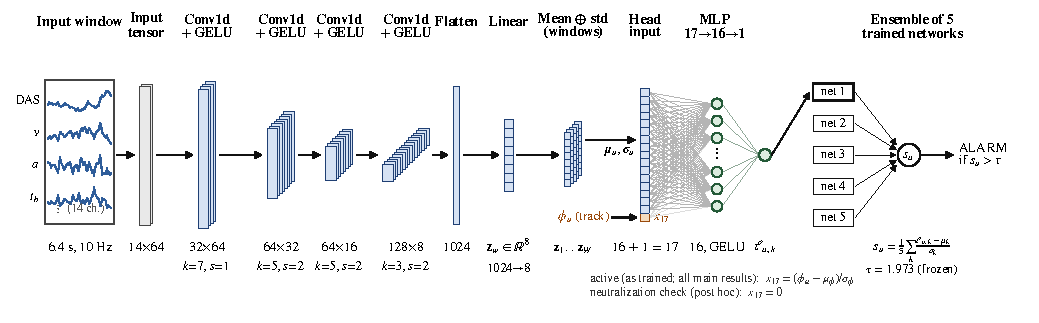
\includegraphics[width=\textwidth]{G0_architecture_two_options}
\caption{\EDIV{} at inference. A 6.4\,s window of the fused track ($14\times64$; left: a real normal window, 4 channels shown) passes four Conv1d+GELU layers (rectangle height $\propto$ time bins, number of rectangles $\propto$ channels; $k$ kernel, $s$ stride), a flatten and a linear projection to $\mathbf z_w\in\mathbb R^8$. The codes of all windows of a track are pooled into mean and standard deviation (16 learned features); one physical summary, the tailgating fraction $\phi_u$, is the 17th input of the trained 17--16--1 head. Five independently trained networks are standardised with frozen $\mu_k,\sigma_k$ and averaged. The 17th input $x_{17}$ (amber) is the standardised $\phi_u$ in the model as trained and tested (all main results) and 0 in the post-hoc neutralized option (\S\ref{sec:q4}). No truth channel is an input.}\label{fig:pipe}\end{figure*}

\section{Data and evaluation}\label{sec:data}
\textbf{Sources.} Everything comes from SimStudio, used unchanged. The simulator steps at 50\,Hz; the DAS model emits detections at 30\,Hz, cameras at 10\,Hz with drops, GPS at 1\,Hz; a Kalman filter per track fuses them into 50\,Hz state rows. Simulator truth is dropped at import and used only to \emph{label} vehicles and to verify that an injected anomaly actually happened. The tracker itself may draw on truth for association and initialisation, which affects all detectors equally (\S\ref{sec:concl}).
\textbf{Network input.} Rows are averaged into 0.1\,s bins (10\,Hz) and map-matched to the lane: eight kinematic channels (longitudinal speed and acceleration, lateral offset and velocity, speed-limit ratio, gap, time headway and closing speed to the vehicle ahead), five sensor-presence masks and the DAS log-amplitude, 14 channels in all. A track is usable with $\ge32$ valid bins and a label-free quality gate.
\textbf{Normal driving and splits.} 1{,}775 exports (148 map regions $\times$ 12 traffic/coverage scenario types, one missing), 14{,}423 tracks. Regions are split spatially with a one-tile buffer: 98 for training, 21 for model selection (val\_A), 21 for thresholds only (val\_B) and 8 for the final test.
\textbf{Anomalies and labels.} Nine types: speeding, reckless, hard braking, stalled, weaving, straddling, tailgating, collision, overweight. An injected vehicle is labelled only if a truth rule confirms the effect (a stop of $\ge10$\,s is a stall; a \emph{legitimate} stop lasts $\ge1$\,s and $<10$\,s with deceleration $<4$\,m/s$^2$ and is labelled normal; tailgating is headway $<0.8$\,s for $\ge5$\,s). Unrealised runs are excluded, never relabelled. The anomaly sets built during the project are introduced where they are used (\S\ref{sec:q}).
\textbf{Evaluation roles.} Results are kept in four classes: \dev{} (nine diagnostic cases, one per type, used for design), \val{} (selection regions, used to choose models), the \ft{} (8 held-out regions, plan frozen before simulation, run once; independent only for the three detectors frozen before it) and \emph{post-hoc} analyses defined after the test was exposed.
\textbf{Decisions and metrics.} The deployment unit is a usable track; a track with fewer than 3 windows gets no decision, and undecided vehicles never count as normal. On the final test a vehicle is detected if any decided track alarms. We report recall per type and macro recall (their mean) at the frozen threshold, ROC-AUC and AUPRC of the pooled anomalies against normal driving, and false alarms on normal driving and on legitimate stops; detectors are compared on the vehicles decided by all of them.

\section{The model: \EDIV}\label{sec:model}
Figure~\ref{fig:pipe} shows the final system. The encoder is the 1-D convolutional encoder of the proposal's autoencoder, pre-trained to reconstruct normal windows and then fine-tuned with the head. A usable track is cut into windows of $T=64$ bins (6.4\,s) with stride 8; the encoder maps each window to an 8-d code. For a unit $u$ (one track in deployment; all tracks of one simulated vehicle in the \dev{}/\val{} tables) the codes are pooled into their mean and standard deviation, standardised with constants fitted on training normals, concatenated with one explicit physical summary, the tailgating fraction $\phi_u$ (share of valid bins with a leader, headway $<0.8$\,s and speed $>5$\,m/s, computed from the tracks, not from truth), and passed to a small MLP head that outputs a logit $\ell_u$. Headway and the leader mask are also encoder inputs, so $\phi_u$ summarises over the whole track what the encoder sees window by window; the model is a hybrid of a learned encoder and this one summary. A fixed preprocessing step removes a tracker artefact (a ``leader'' closer than 1\,m at $>5$\,m/s is a duplicate track). Five seeds $k$ are trained with the same recipe; each logit is standardised by the mean and standard deviation of that seed's logits on the 1{,}242 val\_B normals, and the ensemble score is their mean:
\begin{equation}
 z_{u,k}=\frac{\ell_{u,k}-\mu_k}{\sigma_k},\quad s_u=\frac{1}{5}\sum_{k=1}^{5} z_{u,k},\quad \text{ALARM}\iff s_u>\tau,
\end{equation}
with $\tau=1.9726$ the 99th percentile of $s_u$ on the same val\_B normals, i.e.\ a nominal 1\,\% false-alarm rate. Thresholds come only from val\_B and are never copied between models. Table~\ref{tab:hp} gives the frozen recipe; each seed has 67{,}225 trained parameters.
\textbf{One model, two ways to run it.} The five networks were trained, selected and tested with $\phi_u$ active; all main results belong to this hybrid. The code also offers an explicit \emph{neutralized} option that holds the standardised $\phi_u$ input at 0 on the same weights, $\mu_k$, $\sigma_k$ and $\tau$. It measures how much the trained model depends on $\phi_u$, is not a network trained without $\phi_u$, and was defined after the final test had been exposed (\S\ref{sec:q4}).
\textbf{Baselines.} Two frozen detectors are compared on identical data: the \emph{supervised single model} (one seed, earlier data, no artefact cleaning, no $\phi$; its own val\_B P99) and the \emph{SimStudio Z-score} as shipped (156 features, 13 of which use truth position error; a truth-free variant gives the same macro recall).

\begin{table*}[t]\centering\footnotesize\setlength{\tabcolsep}{3pt}
\caption{Hyper-parameters of the final model (per seed) and of the autoencoder pre-training that initialises its encoder.}\label{tab:hp}
\begin{tabular}{@{}llll@{}}\toprule
Input & 14 channels $\times$ 64 bins (6.4\,s), stride 8 bins & Batch & 48 normal + 16 anomalous vehicles, $\le$32 windows each \\
Encoder & Conv 14--32--64--64--128 (k 7,5,5,3), Linear 1024$\to$8 & Optimiser & AdamW, lr $10^{-4}$ encoder / $10^{-3}$ head, wd $10^{-4}$ \\
Pooling, head & mean$\oplus$std of codes (16) $\oplus\ \phi$; MLP 17--16--1, GELU & Schedule & 120 steps $\times$ $\le$25 epochs, patience 6, grad.\ clip 5 \\
Loss, selection & BCE per vehicle; checkpoint = best validation AP (val\_A) & Training set & 6{,}761 normal / 105 anomalous vehicles ($\ge$3 windows) \\
Ensemble & seeds 0--4; $\mu_k,\sigma_k$ on 1{,}242 val\_B normals; $\tau$ = P99 & Size & 67{,}225 trained parameters per seed \\\midrule
AE pre-training & 14 inputs, 7 masked targets, bounded decoder, masked MSE & AE schedule & AdamW lr $10^{-3}$, batch 256, $\le$100 epochs, pat.\ 10 \\\bottomrule
\end{tabular}\end{table*}

\section{Four questions behind the design}\label{sec:q}
The design was not fixed in advance; each change answered one question with a pre-registered comparison: the data, the single difference between arms and the replacement rule were written before training, and frozen artefacts were hash-checked before and after each round. For each question we give what was compared, the result, the decision and what it does not show; Fig.~\ref{fig:ctrl} shows the comparisons that change one factor. Q1 and Q2 produced the final model; Q3 explains why later candidates with more detections were rejected; Q4, the role of $\phi_u$, uses the exposed test and is answered in \S\ref{sec:q4}. Full records are in the repository (\texttt{research/}, indexed by these questions).

\begin{figure*}[t]\centering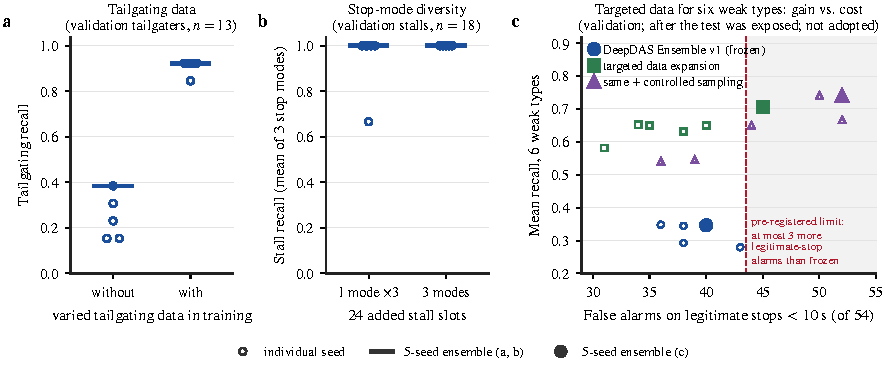
\includegraphics[width=\textwidth]{V5_controlled_comparisons_3panel}
\caption{Controlled comparisons on \val{} data; each panel changes one factor and shows every seed (open) and the five-seed ensemble. (a) Recall on 13 validation tailgaters for the same recipe (with $\phi_u$) trained without and with the varied tailgating data (Q2). (b) Recall on 18 validation stalls (mean over three stop modes) when 24 added stall slots repeat one stop mode or cover three (Q2). (c) Mean recall over the six weak types against false alarms on 54 legitimate stops for the frozen model, the targeted training-data expansion and the same data with controlled sampling; dashed: the pre-registered limit on legitimate-stop alarms (Q3). The models of (c) were trained after the final test had been exposed and were not adopted.}\label{fig:ctrl}\end{figure*}

\subsection*{Q1. Why was reconstruction error not enough, and why supervision?}
\lab{Compared.} The proposed autoencoder (13 channels, $T=64$, 8-d code, P95 window error per track, P99 threshold on val\_B) against the Z-score on the published scenarios and an 81-run severity study (9 types $\times$ 3 levels $\times$ 3 seeds) in held-out regions of the normal corpus: 91 injected and 632 normal vehicles. \lab{Result.} AUROC 0.598 [0.52, 0.67] vs 0.887 [0.84, 0.93]; 1 of 91 injected vehicles at a 1\,\% false-alarm rate vs 44\,\%. The sensitivity analyses promised in the proposal changed nothing: seeds ($\pm0.01$), window length 3.2--12.8\,s and bottleneck 4--32 leave AUROC at 0.58--0.61, and stratifying tracks by their DAS noise level showed no dependence (a noise sweep would have required changing the simulator). A wider code reconstructs normal \emph{and} anomalous windows better. The measurements point to the data: stops, braking up to 4\,m/s$^2$, drift up to 1.8\,m and 1.2\,s headways are all normal driving, so the anomalies lie inside the normal envelope of a 6.4\,s window. A score on the pooled codes instead of the error detected 5 of the 9 original SimStudio scenarios without labels (two through a standstill), though none of the realised braking, straddling or tailgating cases: the codes are informative. A supervised head on the pre-trained encoder, trained on 34 verified anomalies simulated in regions disjoint from evaluation, detected 7 of the 9 \dev{} cases. \lab{Decision.} Keep the encoder, replace the criterion by supervision, which the simulator makes possible because it labels by construction. \lab{Not shown.} Supervision removes the labelling constraint only inside the simulator; the stage-1 numbers come from the archived study report and are not regenerated.

\begin{figure*}[t]\centering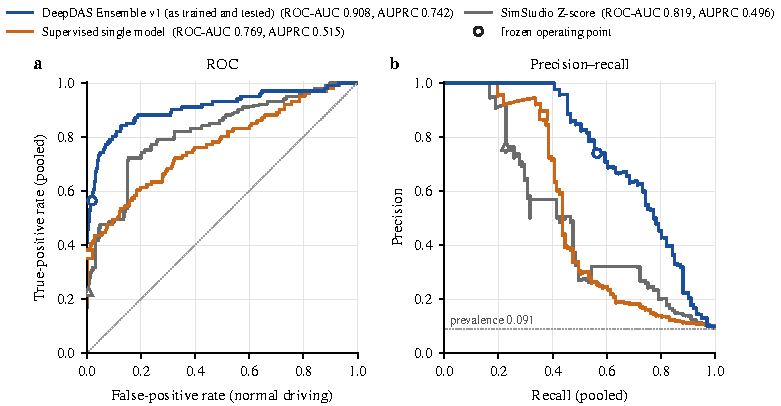
\includegraphics[width=0.8\textwidth]{V6_roc_pr_frozen_detectors}
\caption{Final test, the three detectors frozen before it, common decided subset (101 anomalies, 1{,}008 normal vehicles): (a) ROC, (b) precision--recall; open markers: frozen operating points. The curves rank vehicles; no threshold was chosen from them. The post-hoc neutralized option is summarised in Table~\ref{tab:phi}.}\label{fig:roc}\end{figure*}
\subsection*{Q2. How did training stability and data diversity affect detection?}
\lab{Compared.} Three one-factor comparisons: (i) the supervised recipe with seeds 0--2; (ii) the same five-seed recipe without and with varied tailgating data; (iii) 24 added stall slots that repeat one stop mode or cover three. \lab{Results.} (i) The seeds detected 7, 2 and 3 of the 9 \dev{} cases: with 34 training anomalies the seed alone moved the result by five cases, so from here on five standardised seeds are averaged (Eq.~1) and every comparison is ensemble-level. (ii) Earlier tailgating injections were rarely realised. Four versioned plans produced 59 verified tailgaters on shared planned routes with varied leader speed and episode length, plus matched controls that drive the same route at the default headway; validation tailgating recall rose from 0.385 to 0.923 (Fig.~\ref{fig:ctrl}a). (iii) With the new data the stalled case was missed; tailgating took $\approx$60\,\% of positive draws and all training stalls followed one mode (move--stop 30\,s--move). Type-balanced sampling and a frozen encoder did not restore it. With three stop modes (standing from $t=0$, stop until the end, move--stop--move) every seed detected 18/18 validation stalls, against 0.93 $\pm$ 0.15 per seed when one mode was repeated; diversity also won the tie-break on validation AP (0.781 vs 0.751; Fig.~\ref{fig:ctrl}b). \lab{Decision.} This diversity ensemble became \EDIV{} and was frozen before the final test. \lab{Not shown.} Both tailgating arms included $\phi_u$; no model without $\phi_u$ was trained on the expanded, final training data (Q4).

\begin{figure}[t]\centering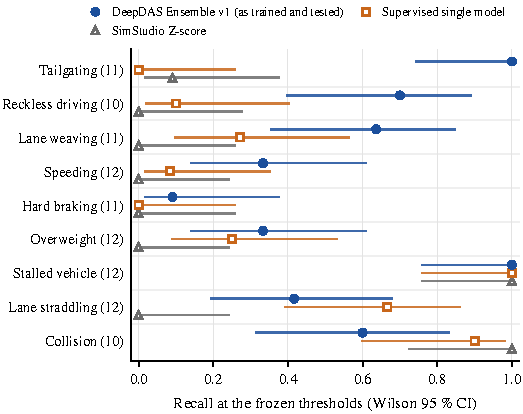
\includegraphics[width=\columnwidth]{V7_detection_by_type_frozen_detectors}
\caption{Final-test recall per anomaly type at the frozen thresholds (common decided subset, $n$ in brackets, Wilson 95\,\% intervals). The ensemble gains on behaviours the Z-score missed; hard braking is weak for every detector (at most 1/11).}\label{fig:type}\end{figure}
\subsection*{Q3. Why do more detections not justify replacing the model?}
\lab{Before the test: legitimate stops.} The selected model flagged 40 of 54 legitimate stops in validation. A read-only diagnosis measured that removing the windows that overlap the truth stop removes every alarm, that the tracker compresses stop duration (a 30\,s truth stop shows $\approx$9\,s), and that training supplied about 105$\times$ fewer stop windows from legitimate stops than from stalls. This supports, without proving it as the only cause, that under mean/std pooling the \emph{share} of stop windows drives the score. \lab{Compared:} three pre-registered remedies on the same data and seeds: controlled exposure to legitimate stops, an added temporal branch over the window sequence, and checkpoint selection by a task rule. \lab{Result:} alarms fell to 37, 27 and 21 of 54, but each variant broke another condition. \lab{Decision:} model unchanged.
\lab{After the test was exposed: weak types.} A read-only diagnosis of the exposed test found the six weak types separable in the input and in the pooled code (linear-probe AUC 0.81--1.0) but less so in the final score, and the head had seen four homogeneous examples per type: this points to the head, without isolating one cause. \lab{Compared:} the frozen model against a targeted training-data expansion (314 new runs, wide parameter grids per weak type, matched legal controls) and the same data with controlled sampling, on an expanded validation set and under nine pre-registered conditions. \lab{Result:} mean weak-type recall rose from 0.35 to 0.71 and 0.74 and ROC-AUC from 0.87 to 0.96; normal-driving false alarms stayed at $\approx$1\,\% and tailgating-control alarms fell (6/7 $\to$ 0/7, 2/7). Both arms passed the other eight conditions, but legitimate-stop alarms rose to 45 and 52 of 54, above the pre-registered limit of 43 (at most three more than the frozen model; Fig.~\ref{fig:ctrl}c). \lab{Decision:} neither was adopted; because the exposed test informed their design, no final-test number exists for them. \lab{Not shown:} with 9--10 validation vehicles per weak type one detection moves recall by 0.1, although every seed of the first arm gains $\ge$0.28. For a road monitor, detections bought with alarms at ordinary stops are not an improvement.

\section{Results}\label{sec:res}
\subsection{Final test}
\textbf{Setup.} 228 runs in the 8 test regions with new scenes, background traffic, seeds and injection lanes; plan, models, thresholds and evaluation code were frozen before simulation, and the test was run once; 105 of 108 core injections were realised. Because coverage differs, Table~\ref{tab:ft} compares the detectors on the vehicles decided by all of them: the deep models decide 1{,}008 of 1{,}708 normal vehicles (134 untracked, 320 without a usable track, 246 with $<3$ windows), the Z-score 1{,}574.
\textbf{Overall.} \EDIV{} reaches macro recall 0.568 against 0.364 and 0.232; paired exact McNemar tests on the pooled anomalies give 38 vs 4 discordant detections against the Z-score ($p<0.001$) and 28 vs 8 against the single model ($p=0.0012$). Its ROC and precision--recall curves lie above both baselines over almost the whole range (Fig.~\ref{fig:roc}).
\textbf{By type} (Fig.~\ref{fig:type}). The gain is on tailgating (11/11) and weaving (7/11), which the Z-score detects 1/11 and 0/11 times, and on reckless driving (7/10); stalls are 12/12 for all three. Hard braking (1/11), speeding (4/12) and overweight (4/12) stay weak; on straddling the single model is better (8/12 vs 5/12), and on collision both baselines are (9/10 and 10/10 vs 6/10).
\textbf{False alarms.} On normal driving 2.0\,\% (1.3\,\% without the tailgating controls), 0.5\,\% and 0.7\,\%; on legitimate stops 20/28 (3\,s 3/8, 5\,s 8/11, 8\,s 9/9), 14/28 and 22/28; on tailgating matched controls 7/11, 0/11 and 0/11, although within each pair the tailgater always scores higher.

\begin{table}[t]\centering\footnotesize\setlength{\tabcolsep}{1.6pt}
\caption{Final test (independent for the three frozen detectors), common decided subset (101 anomalies, 1{,}008 normal vehicles). Macro recall with 95\,\% bootstrap CI over runs. On its own larger decided set (105 anomalies, 1{,}574 normals) the Z-score has ROC-AUC 0.783, AUPRC 0.394, precision 0.64, F1 0.33.}\label{tab:ft}
\begin{tabular}{@{}lccc@{}}\toprule
 & Ens.\ v1 (hybrid) & Single & Z-score \\\midrule
Macro recall & \textbf{0.568} [.49,.65] & 0.364 [.30,.43] & 0.232 [.22,.26] \\
Precision / F1 & 0.74 / \textbf{0.64} & 0.88 / 0.52 & 0.77 / 0.35 \\
ROC-AUC / AUPRC & \textbf{0.908} / \textbf{0.742} & 0.769 / 0.515 & 0.819 / 0.496 \\
FA, normal driving & 20 (2.0\,\%) & 5 (0.5\,\%) & 7 (0.7\,\%) \\
FA, legit.\ stops (of 28) & 20 & 14 & 22 \\
Decided normals of 1{,}708 & 1{,}008 & 1{,}008 & 1{,}574 \\\bottomrule
\end{tabular}\end{table}

\subsection{Development and validation (not independent)}
\textbf{Development.} \EDIV{} detects 8 of the 9 cases; overweight scores 1.865 against $\tau=1.973$. The single model detects 7, missing weaving and tailgating. \textbf{Validation} (used for selection). Macro recall 0.714, AP 0.781, stalls 18/18, tailgating 12/13, false alarms 1.07\,\% on the selection-region normals, legitimate stops 40/54; per-seed macro recall 0.55--0.76.

\subsection{Q4 (post hoc). What does the headway summary add?}\label{sec:q4}
\lab{Why it is there.} When the single model missed the tailgating case, diagnosis showed that headway is an input channel but mean/std pooling does not expose \emph{for how long} it is short, so $\phi_u$ was added as an explicit summary. On the early data it did not help: the development tailgating case stayed undetected with and without it (0/3 seeds each). Both tailgating-data arms of Q2 included it. \lab{Compared.} The frozen hybrid with $\phi_u$ active against the same weights with $\phi_u$ neutralized at inference (Table~\ref{tab:phi}). \lab{Result.} With $\phi_u$ active the model detects one more development case, the tailgating case (score 3.73 vs $-0.08$; its $\phi_u=0.81$ lies 25 standard deviations above the training-normal mean). The other development scores move by $\le$0.03, normal-driving false alarms are unchanged (20/1{,}008), and speeding and collision change by one vehicle each. Most test tailgaters stay detected without $\phi_u$, and a linear probe on the 16 pooled code statistics separates them from normal tracks (AUC 1.0), which suggests that the learned representation carries most of their signal. \lab{Not shown.} This measures dependence, not a network trained without $\phi_u$, and its test rows are post hoc. Whether the tailgating gain came from $\phi_u$, from the data or from both is not identified: no 16-input head was trained on the final training data (early models without $\phi_u$ exist).
\begin{table}[h]\centering\footnotesize\setlength{\tabcolsep}{3pt}
\caption{Q4: dependence of the frozen ensemble on $\phi_u$ (same weights, $\mu_k$, $\sigma_k$ and $\tau$; inference-time intervention).}\label{tab:phi}
\begin{tabular}{@{}lcc@{}}\toprule
Check & $\phi_u$ active (as tested) & $\phi_u$ neutralized \\\midrule
Nine development cases & 8/9 & 7/9 \\
Tailgating, validation & 12/13 & 9/13 \\
Tailgating, exposed test (post hoc) & 11/11 & 10/11 \\
Macro recall, exposed test (post hoc) & 0.568 & 0.560 \\\bottomrule
\end{tabular}\end{table}

\section{Conclusions and limitations}\label{sec:concl}
\textbf{What we learned.} Reconstruction error measures what a bounded, narrow model cannot reproduce; here the anomalies are reproducible within a window. The encoder nevertheless learned a useful representation, and the decisive step was not a new architecture but verified labels, strict separation of regions and scenes, and pre-registered decisions. Twice, diversity of realised examples mattered more than quantity: varied tailgating episodes with matched controls, and three stop modes instead of one.
\textbf{Why some types stay weak.} The tracker's longitudinal acceleration has a median minimum of $-7.5$\,m/s$^2$ on \emph{normal} tracks, stronger than the injected 6\,m/s$^2$ brake, so the brake lies within the range of normal tracks; and normal traffic reaches 1.10--1.12$\times$ the limit, so mild speeding overlaps normal driving by construction. For the other weak types the pooled code separates them better than the final score does (overweight: probe 0.96, score 0.83), which points to the head rather than the encoder (Q3).
\textbf{Real data.} The one real DAS recording (Klausner Street: a bus standing $\approx$31\,s, a stall by our $\ge10$\,s rule) is detected by \EDIV{} in both inference options ($s_u=4.53$ / $4.55>\tau$) and by the Z-score; the stage-1 autoencoder missed it. One case is not a recall estimate.
\textbf{Limitations.} (1) False alarms on legitimate short stops (diagnosed, not removed) and on tailgating matched controls. (2) Weak recall on hard braking, speeding, overweight and straddling; targeted data shows it is learnable, but not within the stop constraint. (3) No decision for 700 of 1{,}708 normal vehicles (41\,\%), set by the tracker and the $\ge3$-window rule. (4) The exported tracks inherit truth through the tracker's association and initialisation, so all detectors see cleaner tracks than a real system would, and there is one real track. (5) The final test is independent only for the three models frozen before it; a later model needs a new test. (6) Severity and sensitivity analyses exist for the autoencoder stage only. (7) The separate contributions of $\phi_u$ and of the tailgating data are not identified.
\textbf{Future work.} A duration-aware stop feature or post-filter computed from the track, a tracker that preserves stop duration, and a labelled real recording; the repository provides the frozen baseline such work must beat.

\balance
\section*{Code and reproducibility}
\url{https://github.com/noasapir3/Deep-DAS} (processed data: release \texttt{data-v1.0}): frozen checkpoints and thresholds, code, published results and the eight study records. \texttt{python scripts/verify\_phi\_modes.py -{}-full} regenerates the development, validation and final-test results in both inference options and compares them with the published files; retraining reproduces the checkpoints bit-exactly on the build platform. Stage-1 and study numbers come from archived records.

\section*{Team contributions}
Noa Sapir led the technical and experimental work, with primary responsibility for designing and generating the simulation scenarios and datasets of this project (building on the SimStudio infrastructure of the earlier project), training the deep-learning models, and executing the experiments. Asaf Zini contributed to preparing and checking simulation inputs and to technical validation of the experimental workflow. Neta Shaboo contributed to the literature review and to organizing and editing the research documentation and report.

\footnotesize
\begin{thebibliography}{9}\setlength{\itemsep}{0pt}
\bibitem{lindsey2021} N.~J. Lindsey and E.~R. Martin, ``Fiber-optic seismology,'' \emph{Annu. Rev. Earth Planet. Sci.}, vol.~49, pp. 309--336, 2021.
\bibitem{ye2023} Z.~Ye \emph{et al.}, ``Traffic flow and vehicle speed monitoring with the object detection method from the roadside distributed acoustic sensing array,'' \emph{Front. Earth Sci.}, vol.~10, 992571, 2023.
\bibitem{robles2025} I.~Robles-Urquijo \emph{et al.}, ``Method to use transport microsimulation models to create synthetic distributed acoustic sensing datasets,'' \emph{Appl. Sci.}, vol.~15, no.~9, 5203, 2025.
\bibitem{sakurada2014} M.~Sakurada and T.~Yairi, ``Anomaly detection using autoencoders with nonlinear dimensionality reduction,'' in \emph{Proc. MLSDA Workshop}, 2014.
\bibitem{audibert2020} J.~Audibert \emph{et al.}, ``USAD: Unsupervised anomaly detection on multivariate time series,'' in \emph{Proc. ACM KDD}, 2020.
\bibitem{ruff2021} L.~Ruff \emph{et al.}, ``A unifying review of deep and shallow anomaly detection,'' \emph{Proc. IEEE}, vol.~109, no.~5, pp. 756--795, 2021.
\bibitem{pang2021} G.~Pang, C.~Shen, L.~Cao, and A.~van den Hengel, ``Deep learning for anomaly detection: A review,'' \emph{ACM Comput. Surv.}, vol.~54, no.~2, 2021.
\bibitem{lakshminarayanan2017} B.~Lakshminarayanan, A.~Pritzel, and C.~Blundell, ``Simple and scalable predictive uncertainty estimation using deep ensembles,'' in \emph{Proc. NeurIPS}, 2017.
\bibitem{wu2023} R.~Wu and E.~Keogh, ``Current time series anomaly detection benchmarks are flawed and are creating the illusion of progress,'' \emph{IEEE Trans. Knowl. Data Eng.}, vol.~35, no.~3, pp. 2421--2429, 2023.
\bibitem{kaufman2012} S.~Kaufman, S.~Rosset, C.~Perlich, and O.~Stitelman, ``Leakage in data mining: Formulation, detection, and avoidance,'' \emph{ACM Trans. Knowl. Discov. Data}, vol.~6, no.~4, 2012.
\end{thebibliography}
\end{document}
